%トランジスタによる論理回路の実現
\chapter{論理回路の実装方法}

\section{簡単な論理回路の実現}
以下のBJTと抵抗を使った回路を考える。
\begin{figure}[htbp]
    \centering
    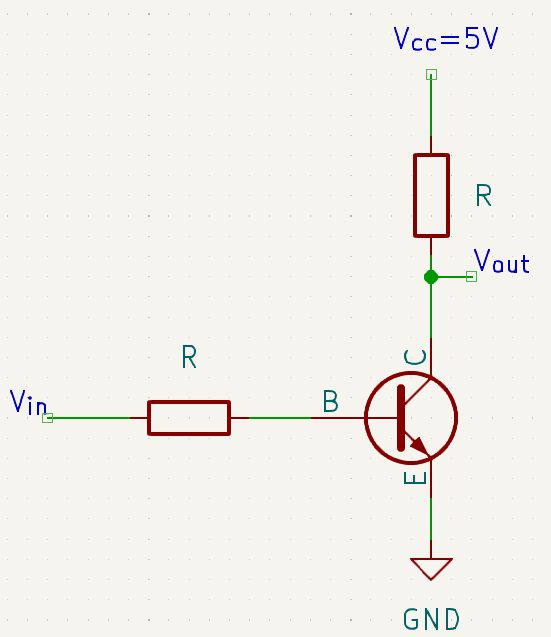
\includegraphics[width=0.3\textwidth]{BJT_logic/logic_circuit.png}
    \caption{}
    \label{fig:logic_circuit}
\end{figure}
この回路において$V_{in}$が0Vであるとき、BJTはベースに電流が流れないため、コレクタ-エミッタ間はとても大きい抵抗となり、$V_{cc}$からGNDに向かって電流が流れないため、
抵抗$R$による電圧降下が発生せず、出力電圧$V_{out}$は$V_{cc}$となる。
一方、$V_{in}$が5Vであるとき、BJTはベースに電流が流れるため、コレクタ-エミッタ間はショートとなり、抵抗$R$によりGNDに向かって電流が流れるため、
抵抗$R$による電圧降下が発生し、出力電圧$V_{out}$は0Vとなる。
以上より、0Vを論理0、5Vを論理1としたとき、以下の真理値表が得られる。
\begin{table}[htbp]
    \centering
    \begin{tabular}{|c|c|}
        \hline
        $V_{in}$ & $V_{out}$ \\
        \hline
        0V (論理0) & 5V (論理1) \\
        5V (論理1) & 0V (論理0) \\
        \hline
    \end{tabular}
    \caption{BJTを用いた論理回路の真理値表}
    \label{tab:logic_circuit_truth_table}
\end{table}
この真理値表はNOT回路の真理値表と一致するため、この回路はNOT回路として動作することがわかる。

ここで考えたいことがある。いま、0Vを論理0、5Vを論理1としたが、これは自明なのだろうか。
実は、0Vを論理1、5Vを論理0とすることも可能である。
電圧を高い状態をH,低い状態をLと表すと、
\begin{align}
  \left\{
    \begin{array}{l}
        L = 0 \\
        H = 1
    \end{array}
    \right.
\end{align}
とするか
\begin{align}
  \left\{
    \begin{array}{l}
        H = 0 \\
        L = 1
    \end{array}
    \right.
\end{align}
とするかの二種類がある。
前者を正論理、後者を負論理と呼ぶ。
この本では、特に断りがない限り正論理を採用する。

とにかく、図\ref{fig:logic_circuit}の回路はNOT回路として動作することがわかった。
また、AND回路やOR回路も図\ref{fig:and_circuit}、図\ref{fig:or_circuit}のようにBJTと抵抗を組み合わせることで実現できる。
\begin{figure}[htbp]
    \begin{minipage}
        {0.45\hsize}
        \centering
        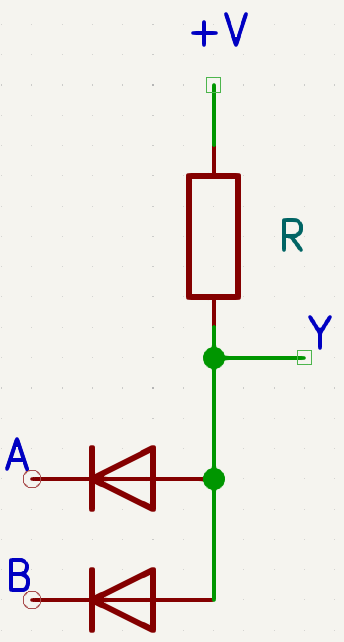
\includegraphics[width=0.4\textwidth]{BJT_logic/and_circuit.png}
        \caption{AND回路}
        \label{fig:and_circuit}
    \end{minipage}
    \begin{minipage}
        {0.45\hsize}
        \centering
        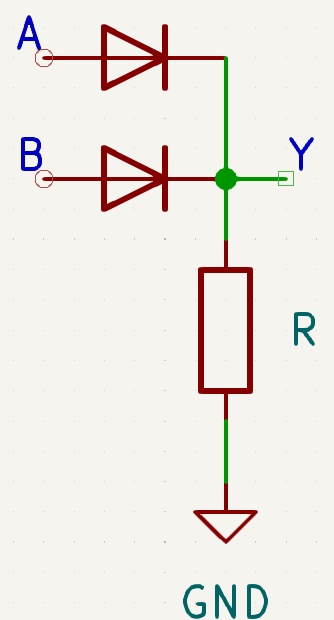
\includegraphics[width=0.4\textwidth]{BJT_logic/or_circuit.png}
        \caption{OR回路}
        \label{fig:or_circuit}
    \end{minipage}
\end{figure}

まず、図\ref{fig:and_circuit}のAND回路について説明する。
AとBの両方が+Vであるとき、ダイオードは導通せず電流は流れないため、抵抗$R$による電圧降下が発生せず、出力電圧$V_{out}$は$V_{cc}$となる。
一方、AまたはBのいずれかが0Vであるとき、対応するダイオードが順方向に導通し、抵抗$R$により0Vの入力に向かって電流が流れるため、抵抗$R$による電圧降下が発生し、出力電圧$V_{out}$は0Vとなる。
よってAND回路の真理値表が得られる。

次に、図\ref{fig:or_circuit}のOR回路について説明する。
AまたはBのいずれかが+Vであるとき、対応するダイオードが順方向に導通し、抵抗$R$によりGNDに向かって電流が流れるため、抵抗$R$による電圧降下が発生し、出力電圧$V_{out}$は$V_{cc}$となる。
一方、AとBの両方が0Vであるとき、ダイオードは導通せず電流は流れないため、抵抗$R$による電圧降下が発生せず、出力電圧$V_{out}$は0Vとなる。
よってOR回路の真理値表が得られる。

しかし、これらの回路には問題点がある。
先ほどまでは無視していたが実際には、ダイオードには空乏層分の電圧降下が存在する。
まずAND回路のほうであるが、Y=Lのとき、ダイオードの空乏層分の電圧が発生してしまうため、Yの電圧が完全に0Vにならない。
次にOR回路のほうであるが、Y=Hのとき、出力電圧がダイオードの空乏層分の電圧だけ低くなってしまうため、Yの電圧が完全に$V_{cc}$にならない。
また、共通の問題として、抵抗に電流が流れ続けるため、電力消費が大きいという問題、負荷によって出力電圧が変動してしまうという問題がある。
よって、現在では、これらの回路はあまり使われておらず、より優れた回路が使われている。



\section{バイポーラトランジスタによる論理回路の実現}

前部の回路の問題点として、出力電圧が完全に0Vまたは$V_{cc}$にならないこと、電力消費が大きいこと、大電流が扱えないこと、
出力インピーダンスが高く負荷によって出力電圧が変動してしまう、入力インピーダンスが低いことが挙げられた。

ひとつづつこれらの問題点を解決していこう。
まず、入力インピーダンスが低いという問題についてであるが、BJTをスイッチとして使うことで解決できる。
図\ref{fig:bjt_logic_circuit}にBJTを用いたNAND回路を示す。
\begin{figure}[htbp]
    \centering
    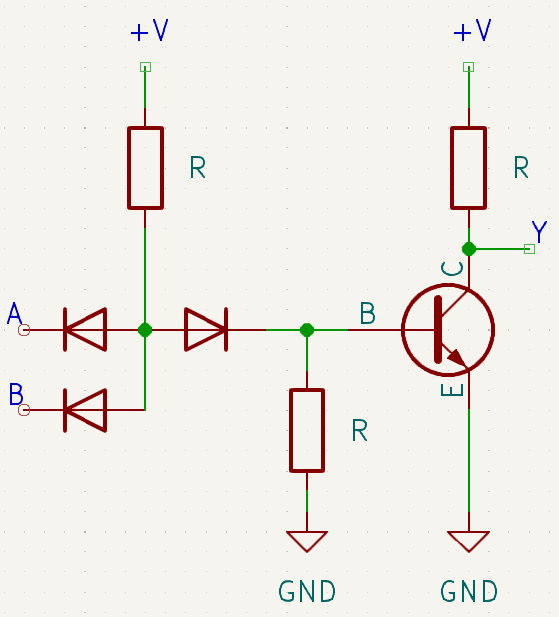
\includegraphics[width=0.3\textwidth]{BJT_logic/bjt_logic_circuit.png}
    \caption{BJTを用いたNAND回路}
    \label{fig:bjt_logic_circuit}
\end{figure}
この回路のようにダイオードとBJTを組み合わせた論理回路のことをダイオード-トランジスタ論理(DTL: Diode-Transistor Logic)回路と呼ぶ。
この回路は前の章のAND回路に反転増幅回路を組み合わせたものであるため、NAND回路として動作することが分かる。
これによって入力インピーダンスの問題に加え、出力電圧が0Vまたは$V_{cc}$にならない問題が解決できた。

次に、大電流が扱えないという問題についてであるが、ダイオードの代わりにBJTを使うことで解決できる。
前章のBJTの理論で余談として述べたが、BJTのベースエミッタ間はダイオードと同様の電流-電圧特性を持つため、ダイオードの代わりにBJTを使うことで大電流を扱うことができる。
トランジスタの量を増やすことに不満があるかもしれないが、結局現在では集積回路としてIC化されているため、ダイオードもトランジスタももはや変わらず、
高速動作性や大電流化のためにBJTを使うことが多い。
ダイオードの代わりにBJTを使う論理回路のことをトランジスタ-トランジスタ論理(TTL: Transistor-Transistor Logic)回路と呼ぶ。

残りの問題は出力インピーダンスと電力消費であるが、これらは出力部に抵抗がついていることが原因である。
この抵抗を取り除き、出力段にトーテムポール回路を採用することで解決できる。

図\ref{fig:ttl_totem_pole}にBJT回路による、TTLトーテムポール出力を有したNAND回路を示す。
\begin{figure}[htbp]
    \centering
    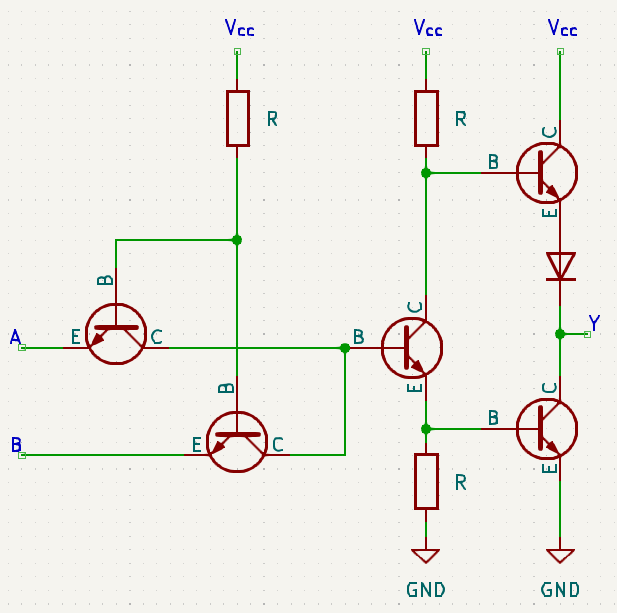
\includegraphics[width=0.5\textwidth]{BJT_logic/ttl_totem_pole.png}
    \caption{TTLトーテムポール出力を有したNAND回路}
    \label{fig:ttl_totem_pole}
\end{figure}

\newpage


この回路の動作を考えよう。
まず、AとBのどちらかが0Vであるとき、対応する入力部のトランジスタがonとなるため、
増幅部(2段目)のトランジスタがoffとなり、出力部(3段目)の上側のトランジスタがon、下側のトランジスタがoffとなる。
そのため、出力電圧$V_{out}$は$V_{cc}$からダイオードの順方向電圧降下分を引いた電圧となる。
一方、AとBの両方が+Vであるとき、入力部のトランジスタがどちらもoffとなるため、
増幅部のトランジスタがonとなり、出力部の上側のトランジスタがoff、下側のトランジスタがonとなる。
そのため、出力電圧$V_{out}$は0Vとなる。
以上より、この回路はNAND回路として動作することが分かる。
これによって出力電圧が完全に0Vまたは$V_{cc}$にならない問題以外の問題は解決できた。
これでNAND回路の実現方法について説明したが、AND回路やOR回路も同様にして実現できる。

また、余談ではあるが、このままの回路であると、出力部の上側と下側のトランジスタが同時にonとなる可能性があり、その瞬間$V_{cc}$からGNDに向かって大電流(貫通電流)が流れてしまう。
これを防ぐために、出力部の上側のトランジスタのコレクタ側に小さめの抵抗(130$\Omega$程度)を挿入することが多い。

以上より、BJTを用いた論理回路の実現方法について説明した。
しかし実は現在では、BJTを用いた論理回路はあまり使われておらず、MOSFETを用いた論理回路が主流となっている。
次章ではMOSFETを用いた論理回路の実現方法について説明する。

